\chapter{Qt framework structure}\label{section:qtstructure}
Qt framework itself is a huge software collection and needs to be divided into logical units. Two main units are \textit{libraries} and \textit{additional software}.

Additional software includes compilers, tools for internationalization and tens of other tools. Some of them will be described in \autoref{section:compilation}.

Let's dig into Qt libraries now. Qt offers very rich and diverse functionality (see \autoref{section:components}), ranging from network communication to painting vector pictures.

\section{Modules}
Each unit of related functionality is called \textit{module}\index{module}. Module is set of classes which is contained within the single (static or dynamic, see \autoref{section:compilation}) library file. If you want to use this module in your code, then you have to include appropriate header files and link your binary against the library file. More modules you need results in more linked libraries and bigger output binaries. Choice of Qt modules for application programming is therefore important.

\subsection{Linking}\label{listing:linking}
Each module usually depends on QtCore\index{QtCore} module, including QtWidgets module. Moreover, QtWidgets module depends on QtGui module. So each Qt-based application with user interface has to be linked against 3 or more modules.

Consider elementary \fdocabbrevref{GUI} application with main window. You can find source in\fdocinlinecode{text}{!}{sources/laboratory/04-guiapp} subdirectory. Application is compiled with modules QtCore and QtWidgets. You can use GNU \textit{ldd}\index{ldd} application to list all dynamic libraries required for executable file to run successfully. Output for our sample application looks very similar to the on in \autoref{listing:ldd}.

\begin{fdoccode}{text}{listing:ldd}{Libraries needed for \fdocabbrevref{GUI} application}
[root@arch-linux 04-guiapp]# ldd -d -r 04-guiapp
linux-gate.so.1 (0xb77c7000)
libQt5Widgets.so.5 => /opt/qt5/5.0.0/gcc/lib/libQt5Widgets.so.5 (0xb719f000) (*@\label{listing:qt5w}@*)
libQt5Gui.so.5 => /opt/qt5/5.0.0/gcc/lib/libQt5Gui.so.5 (0xb6d89000)
libQt5Core.so.5 => /opt/qt5/5.0.0/gcc/lib/libQt5Core.so.5 (0xb693f000) (*@\label{listing:qt5c}@*)
libGL.so.1 => /usr/lib/libGL.so.1 (0xb6833000)
libpthread.so.0 => /usr/lib/libpthread.so.0 (0xb6817000)
libstdc++.so.6 => /usr/lib/libstdc++.so.6 (0xb672e000)
libm.so.6 => /usr/lib/libm.so.6 (0xb66eb000)
libgcc_s.so.1 => /usr/lib/libgcc_s.so.1 (0xb66ce000)
libc.so.6 => /usr/lib/libc.so.6 (0xb651d000)
libgobject-2.0.so.0 => /usr/lib/libgobject-2.0.so.0 (0xb64cd000)
libglib-2.0.so.0 => /usr/lib/libglib-2.0.so.0 (0xb63d2000)
libX11.so.6 => /usr/lib/libX11.so.6 (0xb629c000)
libicui18n.so.49 => /opt/qt5/5.0.0/gcc/lib/libicui18n.so.49 (0xb6084000)
libicuuc.so.49 => /opt/qt5/5.0.0/gcc/lib/libicuuc.so.49 (0xb5f0a000)
libdl.so.2 => /usr/lib/libdl.so.2 (0xb5f05000)
libgthread-2.0.so.0 => /usr/lib/libgthread-2.0.so.0 (0xb5f01000)
librt.so.1 => /usr/lib/librt.so.1 (0xb5ef8000)
/lib/ld-linux.so.2 (0xb77c8000)
libXext.so.6 => /usr/lib/libXext.so.6 (0xb5ee5000)
libpcre.so.1 => /usr/lib/libpcre.so.1 (0xb5e7d000)
libffi.so.6 => /usr/lib/libffi.so.6 (0xb5e76000)
libxcb.so.1 => /usr/lib/libxcb.so.1 (0xb5e53000)
libicudata.so.49 => /opt/qt5/5.0.0/gcc/lib/libicudata.so.49 (0xb4d32000)
libXau.so.6 => /usr/lib/libXau.so.6 (0xb4d2e000)
libXdmcp.so.6 => /usr/lib/libXdmcp.so.6 (0xb4d27000)
\end{fdoccode}

Pay attention to lines \ref{listing:qt5w} -- \ref{listing:qt5c}. Typical program with user interface needs to be linked against QtCore, QtGui and QtWidgets. Console applications need just QtCore. You can list unused (but linked) libraries too as seen in \autoref{listing:ldd2}.

\begin{fdoccode}{text}{listing:ldd2}{Unused (but linked) libraries for \fdocabbrevref{GUI} application}
[root@arch-linux 04-guiapp]# ldd -d -r -u 04-guiapp
Unused direct dependencies:
/opt/qt5/5.0.0/gcc/lib/libQt5Gui.so.5
/usr/lib/libGL.so.1
/usr/lib/libpthread.so.0
/usr/lib/libm.so.6
\end{fdoccode}

Threading library (pthread\index{pthread}) is used by QtCore on Linux. LibGL\index{libGL} is 3D graphics library. LibGL is unused because no OpenGL-related\index{OpenGL} function was called explicitly in our sample application. You will learn more about linking in \autoref{section:compilation}.

Number of chosen modules affects memory consumption an executable file. So pick a reasonable subset of available Qt modules to make your application thin and fit.

\begin{fdocextra}
There are two types of library linkage:
\begin{description}
\item[DYNAMIC LINKAGE] \hfill \\
Is very popular for its usefulness. Dynamic linking\index{dynamic linkage} means that executable file (operating system more precisely) seeks for needed libraries in certain predefined paths in run time. Usually one version of each library is placed somewhere in well-known folder structure and each executable is linked against it. So more running executables can actually use the same library file. This saves memory and is very popular within Unix-like operating systems but it can bring certain level of disorder into poorly designed operating system. This has something to do with Windows because many applications doesn't link with libraries stored in system path and use varying versions of the same library sometimes, duplicating library presence in memory and increasing memory usage.
\item[STATIC LINKAGE] \hfill \\
Not so favourite kind of linkage. Library is packed into executable file and linked in compile time. This makes executable file (sometimes considerably) larger but no additional dependencies (in form of external dynamic libraries) are required. GNU GPL\index{GNU GPL} Qt libraries \textbf{cannot} be linked statically.
\end{description}
\end{fdocextra}

\section{Tree-like class structure}
Cleverly developed library has smart class structure which makes that library easily maintainable, expandable and functional. \textit{Class inheritance}\index{class inheritance} is used very extensively if library design is something we need to deal with. Read \citep[p.~708-783]{prata:cprimer} to get more familiar with \cpp class inheritance if you are not so far. Class inheritance says that if one class is inheritor of another class, then it inherits parent's \textit{data} and \textit{methods}.

It's good practice to have some properties available in all classes of the library. Such a property could be \eg \textit{id}, the textual (or perhaps numerical) identification of each object (instantiated class) within the library. You would have to define what \textit{id} means in each and every of your classes manually without inheritance usage. With inheritance, everything you must do, is to define \textit{id} in exactly one of your classes, promoting this class to \textit{root} class and make rest of classes to inherit the new \textit{library base class}.

This approach is solid base for having library with the tree-like structure (see \autoref{figure:library}) where classes are structured according to their natural relationship.

So, as we found out, there is exactly one class that sits above other classes, which share its data and methods. Qt disposes this kind of top-level class too, it's called\fdocinlinecode{cpp}{!}{QObject}.

\begin{fdocextra}
Many well-known libraries follow root class idea and tree-like class structure. One example is .NET Framework. Its very base class is called\fdocinlinecode{csharp}{!}{System.Object} and provides some basic functionality (shared by all .NET classes via class inheritance) such as method providing basic string representation of each object. You can find more about .NET base class in \citep[p.~84]{nigel:csharp}. Java follows very similar class hierarchy ideas.
\end{fdocextra}

\begin{figure}[ht]
\centering
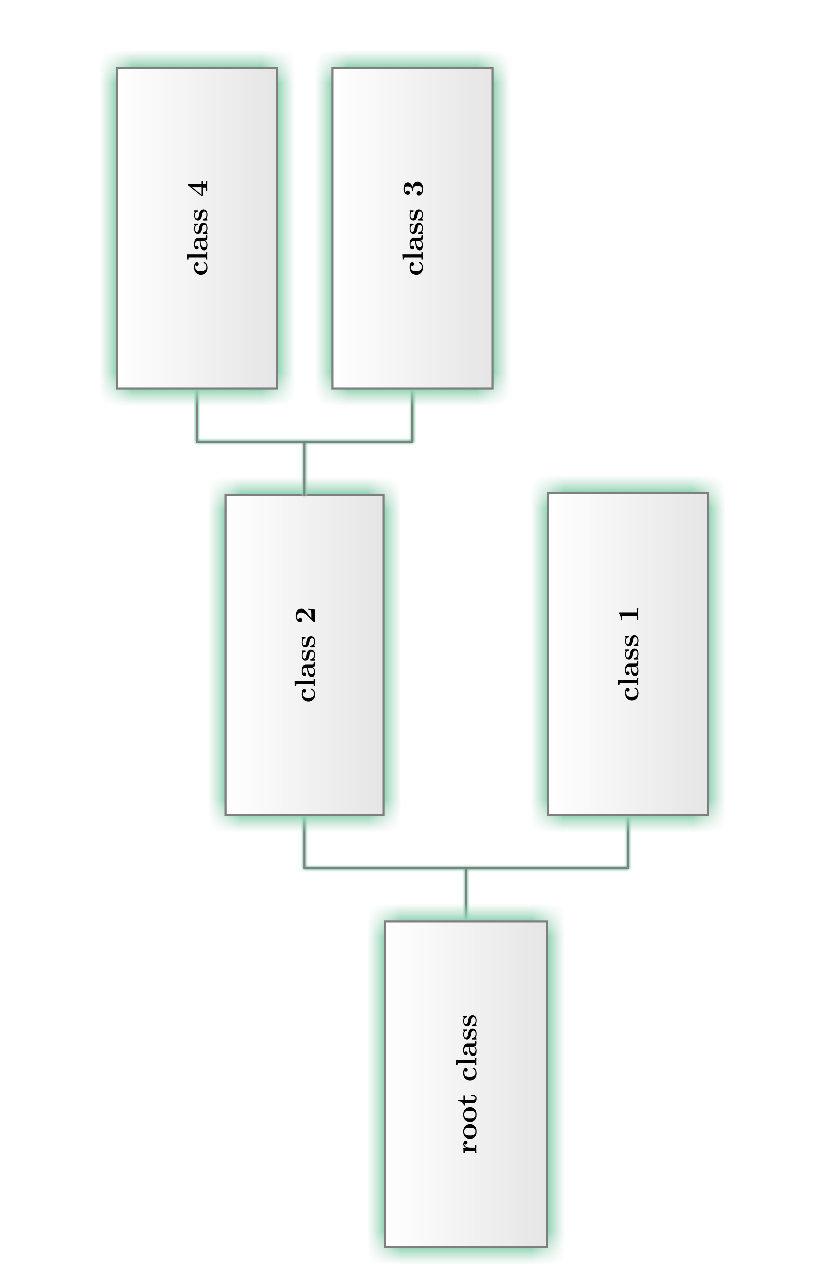
\includegraphics[angle=-90,width=14cm]{graphics/laboratory/02-tree.pdf}
\caption{Typical library tree-like class structure}\label{figure:library}
\end{figure}